%%%%%%%%%%%%%%%%%%%%%%%%%%%%%%%%%%%%%%%%%%%%%%%%%%%%%%%%%%%%%%%%%%%%%%%%
\chapter{CamemBERT}\label{appendix:camembert}
%%%%%%%%%%%%%%%%%%%%%%%%%%%%%%%%%%%%%%%%%%%%%%%%%%%%%%%%%%%%%%%%%%%%%%%%

\begin{table}[ht]
    \small\centering
    \scalebox{0.65}{
        \begin{tabular}{ l l c c c  c @{\hspace{0.35cm}}  @{\hspace{0.35cm}} c  c @{\hspace{0.35cm}}  @{\hspace{0.35cm}} c  c  @{\hspace{0.35cm}}  @{\hspace{0.35cm}} c  c @{\hspace{0.35cm}}  @{\hspace{0.35cm}} c @{\hspace{0.35cm}}  @{\hspace{0.35cm}} c }
            \toprule
                                                    &                                         &                                       &                                         & \multicolumn{2}{c @{\hspace{0.5cm}}}{\textsc{GSD}} & \multicolumn{2}{c @{\hspace{0.7cm}}}{\textsc{Sequoia}} & \multicolumn{2}{c @{\hspace{0.7cm}}}{\textsc{Spoken}} & \multicolumn{2}{c @{\hspace{0.7cm}}}{\textsc{ParTUT}} & \textsc{NER}      & \textsc{NLI}                                                                                      \\
            \cmidrule(l{2pt}r{0.4cm}){5-6}\cmidrule(l{-0.2cm}r{0.4cm}){7-8}\cmidrule(l{-0.2cm}r{0.4cm}){9-10}\cmidrule(l{-0.2cm}r{0.4cm}){11-12}\cmidrule(l{-0.2cm}r{0.4cm}){13-13} \cmidrule(l{-0.2cm}r{2pt}){14-14}
            \multirow{-2}{*}[2pt]{\textsc{Dataset}} & \multirow{-2}{*}[2pt]{\textsc{Masking}} & \multirow{-2}{*}[2pt]{\textsc{Arch.}} & \multirow{-2}{*}[2pt]{\textsc{\#Steps}} & \textsc{UPOS}                                      & \textsc{LAS}                                           & \textsc{UPOS}                                         & \textsc{LAS}                                          & \textsc{UPOS}     & \textsc{LAS}      & \textsc{UPOS}     & \textsc{LAS}      & \textsc{F1}       & \textsc{Acc.}     \\
            \midrule

            \multicolumn{11}{l}{\hspace*{6mm}\em Fine-tuning}                                                                                                                                                                                                                                                                                                                                                                                                                                                                         \\[0.5mm]
            \toprule
            OSCAR                                   & Subword                                 & \textsc{Base}                         & 100k                                    & \textbf{98.25}                                     & 92.29                                                  & \underline{99.25}                                     & 93.70                                                 & 96.95             & 79.96             & \underline{97.73} & \textbf{92.68}    & 89.23             & 81.18             \\
            OSCAR                                   & Whole-word                              & \textsc{Base}                         & 100k                                    & \underline{98.21}                                  & 92.30                                                  & 99.21                                                 & \underline{94.33}                                     & 96.97             & 80.16             & \textbf{97.78}    & 92.65             & 89.11             & 81.92             \\
            CCNET                                   & Subword                                 & \textsc{Base}                         & 100k                                    & 98.02                                              & 92.06                                                  & \textbf{99.26}                                        & 94.13                                                 & 96.94             & 80.39             & 97.55             & \underline{92.66} & 89.05             & 81.77             \\
            CCNET                                   & Whole-word                              & \textsc{Base}                         & 100k                                    & 98.03                                              & \underline{\textbf{92.43}}                             & 99.18                                                 & 94.26                                                 & \underline{96.98} & \underline{80.89} & 97.46             & 92.33             & \underline{89.27} & 81.92             \\
            CCNET                                   & Whole-word                              & \textsc{Base}                         & 500k                                    & \underline{98.21}                                  & \underline{\textbf{92.43}}                             & 99.24                                                 & \textbf{94.60}                                        & 96.69             & \textbf{80.97}    & 97.65             & 92.48             & 89.08             & \underline{83.43} \\
            CCNET                                   & Whole-word                              & \textsc{Large}                        & 100k                                    & 98.01                                              & 91.09                                                  & 99.23                                                 & 93.65                                                 & \textbf{97.01}    & \underline{80.89} & 97.41             & 92.59             & \textbf{89.39}    & \textbf{85.29}    \\


            \midrule
            \multicolumn{11}{l}{\hspace*{6mm}\em Embeddings (with UDPipe Future (tagging, parsing) or LSTM+CRF (NER))}                                                                                                                                                                                                                                                                                                                                                                                                                \\[0.5mm]
            OSCAR                                   & Subword                                 & \textsc{Base}                         & 100k                                    & \underline{\textbf{98.01}}                         & 90.64                                                  & \textbf{99.27}                                        & 94.26                                                 & \underline{97.15} & \textbf{82.56}    & \textbf{97.70}    & \underline{92.70} & \textbf{90.25}    & -                 \\
            OSCAR                                   & Whole-word                              & \textsc{Base}                         & 100k                                    & 97.97                                              & 90.44                                                  & \underline{99.23}                                     & 93.93                                                 & 97.08             & 81.74             & 97.50             & 92.28             & 89.48             & -                 \\
            CCNET                                   & Subword                                 & \textsc{Base}                         & 100k                                    & 97.87                                              & \textbf{90.78}                                         & 99.20                                                 & \underline{94.33}                                     & \textbf{97.17}    & \underline{82.39} & \underline{97.54} & 92.51             & 89.38             & -                 \\
            CCNET                                   & Whole-word                              & \textsc{Base}                         & 100k                                    & 97.96                                              & \underline{90.76}                                      & \underline{99.23}                                     & \textbf{94.34}                                        & 97.04             & 82.09             & 97.39             & \textbf{92.82}    & \underline{89.85} & -                 \\
            CCNET                                   & Whole-word                              & \textsc{Base}                         & 500k                                    & 97.84                                              & 90.25                                                  & 99.14                                                 & 93.96                                                 & 97.01             & 82.17             & 97.27             & 92.28             & 89.07             & -                 \\
            CCNET                                   & Whole-word                              & \textsc{Large}                        & 100k                                    & \underline{\textbf{98.01}}                         & 90.70                                                  & \underline{99.23}                                     & 94.01                                                 & 97.04             & 82.18             & 97.31             & 92.28             & 88.76             & -                 \\
            % ablation : 
            % %% ["10125734", "10126431", "10126429", "10126640","10126641"] # 
            % large ls_pos = ["10129280","10129224"]+["10129215", "10129223"]
            % ls_long = ["10129339", "10129416", "10129415", "10129415"]
            %  ls_long gsd :  ["10129611"] ( 2 seeds only) 
            \bottomrule
        \end{tabular}}
    \caption{Performance reported on \textbf{Test sets} for all trained models (\textbf{average} over multiple fine-tuning seeds).}
    \label{tab:all_results}
\end{table}

In this appendix, we analyze different design choices of \camembert (Table~\ref{tab:ablation}), namely with respect to the use of whole-word masking, the training dataset, the model size, and the number of training steps in complement with the analyses of the impact of corpus origin and size (Section~\ref{sec:origin_and_size}). In all the ablations, all scores come from at least 4 averaged runs. For POS tagging and dependency parsing, we average the scores on the 4 treebanks. We also report all averaged test scores of our different models in Table~\ref{tab:all_results}.

\begin{table}[!htbp]
    \centering\small
        \begin{tabular}{lcccc @{\hspace{0.7cm}} cccc}
            \toprule
            \textsc{Dataset}     & \textsc{Masking}          & \textsc{Arch.}               & \#\textsc{Param.}   & \#\textsc{Steps}    & \textsc{UPOS}  & \textsc{LAS}   & \textsc{NER}   & \textsc{XNLI}  \\
            \midrule
            \multicolumn{9}{l}{\hspace*{6mm}\em Masking Strategy}                                                                                                                                           \\
            {\color{gray}\oscar} & Subword                   & {\color{gray}\textsc{Base}}  & {\color{gray}110M}  & {\color{gray}100k}  & 97.78          & 89.80          & \textbf{91.55} & 81.04          \\
            {\color{gray}\oscar} & Whole-word                & {\color{gray}\textsc{Base}}  & {\color{gray}110M}  & {\color{gray}100k}  & \textbf{97.79} & \textbf{89.88} & 91.44          & \textbf{81.55} \\
            \midrule
            \multicolumn{9}{l}{\hspace*{6mm}\em Model Size}                                                                                                                                                 \\
            {\color{gray}\ccnet} & {\color{gray}Whole-word}  & \textsc{Base}                & 110M                & {\color{gray}100k}  & 97.67          & 89.46          & 90.13          & 82.22          \\
            {\color{gray}\ccnet} & {\color{gray} Whole-word} & \textsc{Large}               & 335M                & {\color{gray} 100k} & \textbf{97.74} & \textbf{89.82} & \textbf{92.47} & \textbf{85.73} \\
            \midrule
            \multicolumn{9}{l}{\hspace*{6mm}\em Dataset}                                                                                                                                                    \\
            \ccnet               & {\color{gray} Whole-word} & {\color{gray}\textsc{Base}}  & {\color{gray}110M}  & {\color{gray}100k}  & 97.67          & 89.46          & 90.13          & \textbf{82.22} \\
            \oscar               & {\color{gray} Whole-word} & {\color{gray}\textsc{Base}}  & {\color{gray}110M}  & {\color{gray}100k}  & \textbf{97.79} & \textbf{89.88} & \textbf{91.44} & 81.55          \\
            \midrule
            \multicolumn{9}{l}{\hspace*{6mm}\em Number of Steps}                                                                                                                                            \\
            {\color{gray}\ccnet} & {\color{gray} Whole-word} & {\color{gray} \textsc{Base}} & {\color{gray} 110M} & 100k                & \textbf{98.04} & 89.85          & 90.13          & 82.20          \\
            {\color{gray}\ccnet} & {\color{gray} Whole-word} & {\color{gray} \textsc{Base}} & {\color{gray} 110M} & 500k                & 97.95          & \textbf{90.12} & 91.30          & \textbf{83.04} \\
            \bottomrule
        \end{tabular}
    \caption{Comparing scores on the \textbf{Validation sets} of different design choices. POS tagging and parsing datasets are averaged. (average over multiple fine-tuning seeds).
        \label{tab:ablation}}
\end{table}


\section{Impact of Whole-Word Masking}
In Table~\ref{tab:ablation}, we compare models trained using the traditional subword masking with whole-word masking. Whole-Word Masking positively impacts downstream performances for NLI (although only by 0.5 points of accuracy). To our surprise, this Whole-Word Masking scheme does not benefit much lower level task such as Name Entity Recognition, POS tagging and Dependency Parsing.

\section{Impact of model size}
Table~\ref{tab:ablation} compares models trained with the BASE and LARGE architectures. These models were trained with the \ccnet corpus (135 GB) for practical reasons. We confirm the positive influence of larger models on the NLI and NER tasks. The LARGE architecture leads to respectively 19.7\% error reduction and 23.7\%. To our surprise, on POS tagging and dependency parsing, having three time more parameters doesn't lead to a significant  difference compared to the BASE model. \citet{tenney-etal-2019-bert} and \citet{jawahar-etal-2019-bert} have shown that low-level syntactic capabilities are learned in lower layers of \bert while higher level semantic representations are found in upper layers of \bert. POS tagging and dependency parsing probably do not benefit from adding more layers as the lower layers of the BASE architecture already capture what is necessary to complete these tasks.

\section{Impact of training dataset}

Table~\ref{tab:ablation} compares models trained on \ccnet and on \oscar.
The major difference between the two datasets is the additional filtering step of \ccnet that favors Wikipedia-Like texts.
The model pretrained on \oscar gets slightly better results on POS tagging and dependency parsing, but gets a larger +1.31 improvement on NER.
The \ccnet model gets better performance on NLI (+0.67).

\section{Impact of number of steps}
\label{sec:nbsteps}

\begin{figure}[t]
    \centering
    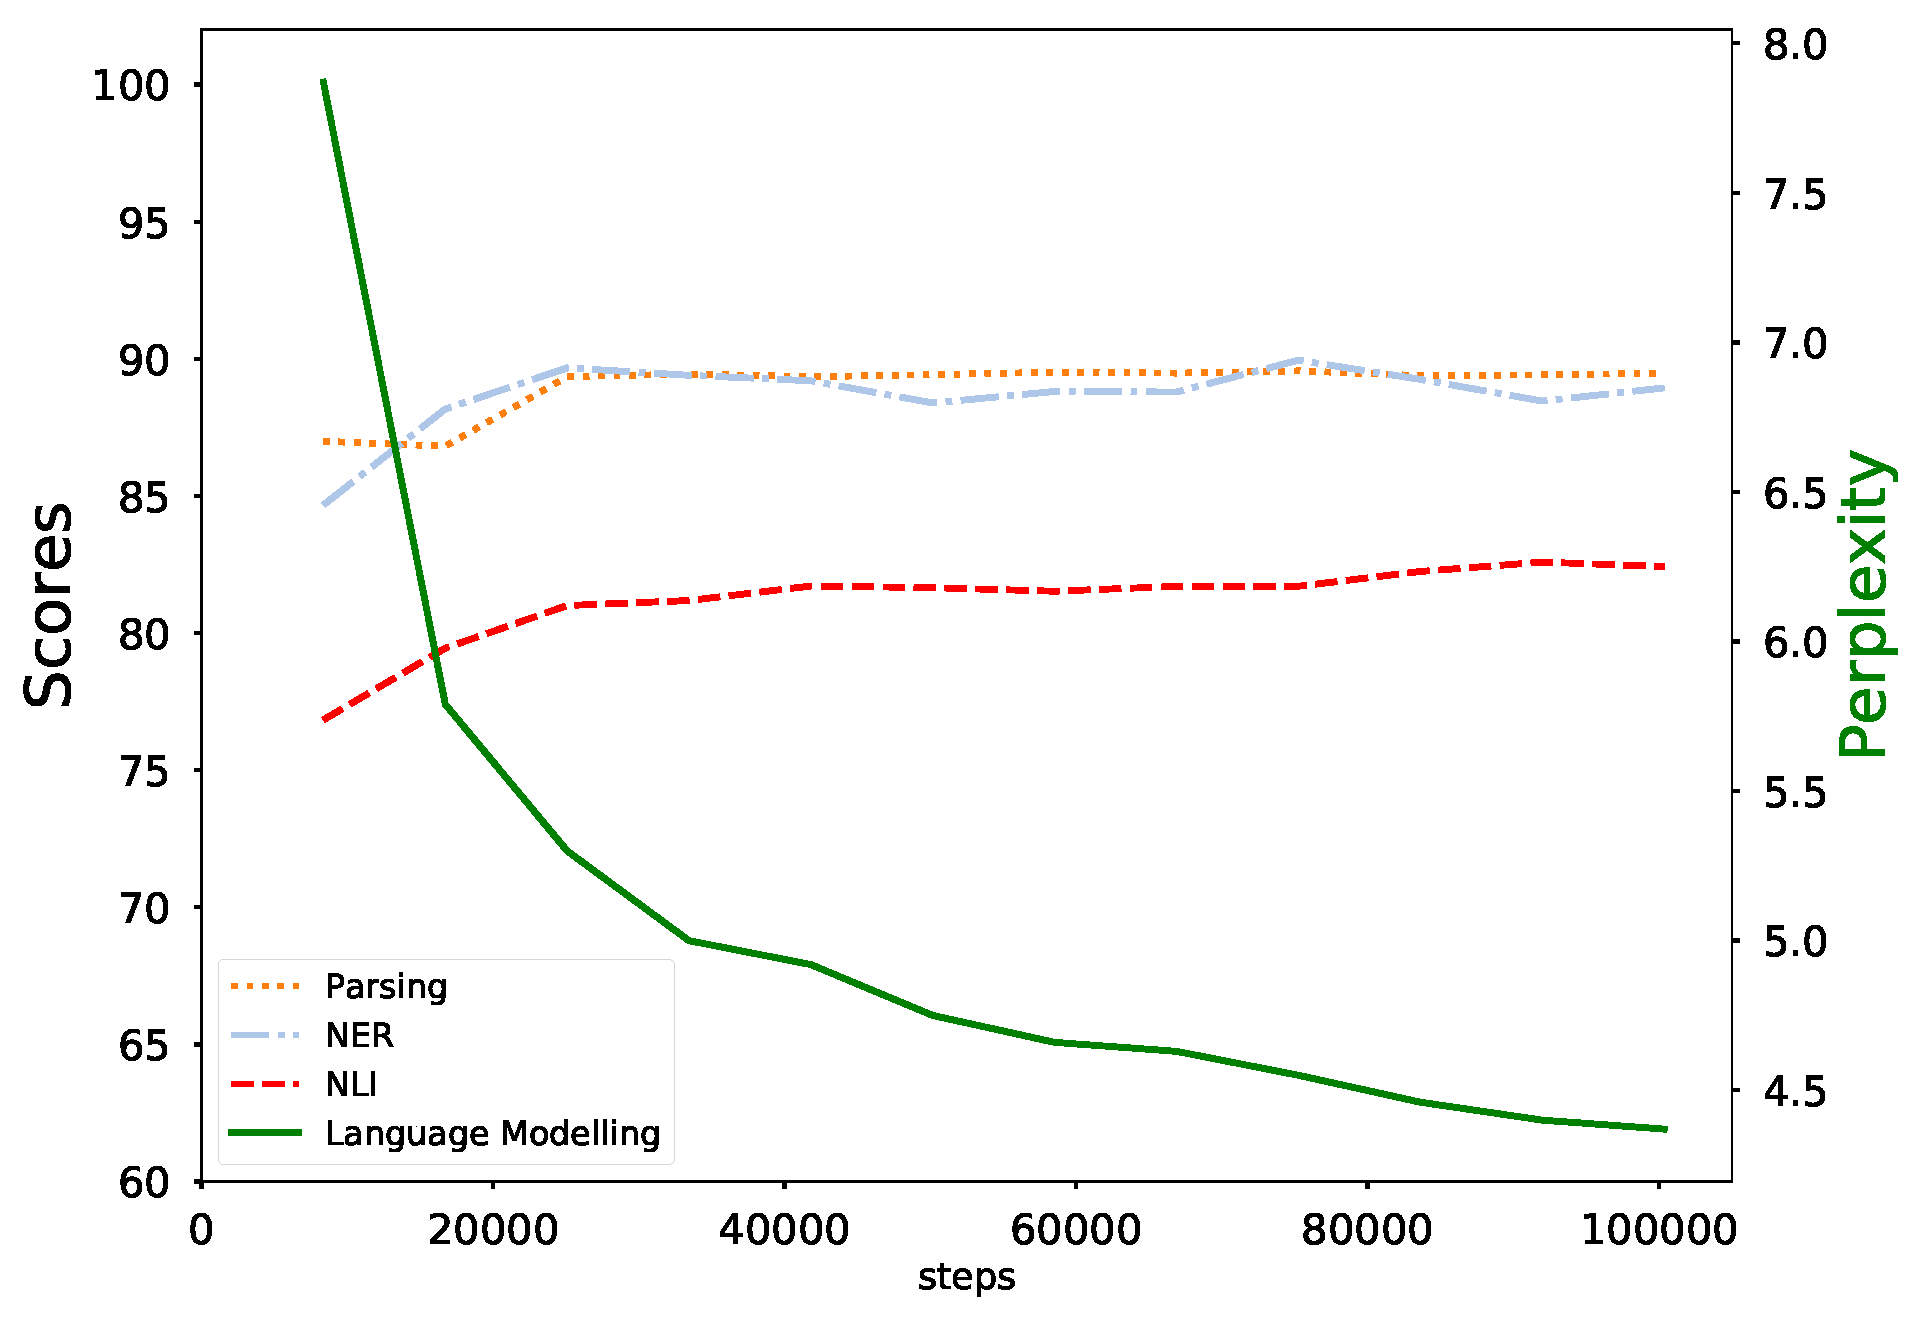
\includegraphics[width=0.75\linewidth]{static/media/mod_eval/camembert/plot_steps_impact_4.pdf}
    \caption{Impact of number of pretraining steps on downstream performance for \camembert.}.
    \label{fig:n_steps_impact}
\end{figure}


Figure~\ref{fig:n_steps_impact} displays the evolution of downstream task performance with respect to the number of steps. All scores in this section are averages from at least 4 runs with different random seeds. For POS tagging and dependency parsing, we also average the scores on the 4 treebanks.

We evaluate our model at every epoch (1 epoch equals 8360 steps). We report the masked language modelling perplexity along with downstream performances.
Figure~\ref{fig:n_steps_impact}, suggests that the more complex the task the more impactful the number of steps is. We observe an early plateau for dependency parsing and NER at around 22k steps, while for NLI, even if the marginal improvement with regard to pretraining steps becomes smaller, the performance is still slowly increasing at 100k steps.

In Table~\ref{tab:ablation}, we compare two models trained on \ccnet, one for 100k steps and the other for 500k steps to evaluate the influence of the total number of steps. The model trained for 500k steps does not increase the scores much from just training for 100k steps in POS tagging and parsing.
The increase is slightly higher for XNLI (+0.84).

Those results suggest that low level syntactic representation are captured early in the language model training process while it needs more steps to extract complex semantic information as needed for NLI.